In this chapter the planning and work-flow regarding Sprint 6 will be described. This is the last sprint and it is also of shorter length. Since the implementation of the product is already done this chapter will omit certain sections such as Architecture, Implementation and Testing which are present in the previous fully-fledged sprints chapters. At the end the team will evaluate the whole sprint, and try to answer on following questions: What went well? What could be improved?  

\section{Sprint planning}
It was formerly intended to devote the last sprint to the tasks related with finishing and refining the report as well as preparing the final presentation and rehearsing. Nevertheless as the application performance issues occurring during the last sprint prevented the team from accomplishing to record the final demonstration video part of the total sum of person-hours available in this sprint must be spent on creating the video again.

The planning of this sprint started already during the last customer meeting held on 7th November where he suggested to use different types of imagery to be displayed on borrowed phones (see Section \ref{txt:sprint5_customerfeedback}). One of the tasks therefore should be to create suitable images and/or videos in multiple scales as it was uncertain how many phones would be available during recording. The team members should also try to collect as many mobile devices as possible and also borrow the video recording device.

Next significant part of the sprint should be devoted to creating the demonstration video which would fulfill the requirement to amaze and entertain the viewers. As already planned this sprint will also mainly focus on finalizing and refining the report, preparing it for the submission, creating the final presentation and rehearse.

It should not be forgotten to deploy both server and client side application on Google Play as this is one of the non-functional requirements (see Section \ref{txt:requirements}).

Due to the fact the final version of the project must be submitted on the fixed date this sprint is shorter by two work days and the workload must be adjusted accordingly. The team has eight work days to its disposal which makes it for 140 person-hours for the whole team.

All implementation related stories for sprint 6 are presented in Table \ref{tab:sprint6stories}.
%\caption{User stories selected for Sprint 4.}
  \label{tab:sprint4stories}
 \def\arraystretch{1.25}
 
\begin{longtable}{ccXcc}

\toprule[0.5mm]
\multirow{2}{*}{\textbf{ID}} &
\multirow{2}{*}{\textbf{Ref.}} & \multirow{2}{*}{\textbf{Description}} & \multicolumn{2}{c}{\textbf{Hours}} \\
 					& & & \textbf{Est.} & \textbf{Sp.} \\
%\textbf{ID} 	& \textbf{Description} 	& \textbf{Est.} & \textbf{Sp.} \\
\midrule
\textbf{I4.1} 	& 	& {\bf As a server I need to link the devices' location with their ids.}	 &  52	& \textbf{48} \\

\textbf{I4.2} 	& 	& {\bf As a server I need to identifiy multiple clients from light.}		 &  19	& \textbf{18} \\

\textbf{I4.3} 	& 	& {\bf As a server I need to map all available devices to grid.} 			 & 22 & \textbf{18} \\	

\textbf{I4.4} 	& 	& {\bf As a server I need to play the whole media to the grid.} 			 & 37 & \textbf{34} \\
	
\midrule
		
				&& \textbf{SUM:}		&		130	& \textbf{136}
 \\																			
\bottomrule[0.5mm]
\end{longtable}

All the documentation related stories for sprint 6 are presented in Table \ref{tab:sprint6Documentationstories}. 
%\caption{User stories selected for Sprint 2.}
\def\arraystretch{1.25}
 
\begin{longtable}{ccXcc}
\label{tab:sprint2Documentationstories}\\[-6mm]
\caption{Documentation stories selected for sprint 2}\\[-4mm]
\toprule[0.5mm]
\multirow{2}{*}{\textbf{ID}} &
\multirow{2}{*}{\textbf{Ref.}} & \multirow{2}{*}{\textbf{Description}} & \multicolumn{2}{c}{\textbf{Hours}} \\
 					& & & \textbf{Est.} & \textbf{Sp.} \\
%\textbf{ID} 	& \textbf{Description} 	& \textbf{Est.} & \textbf{Sp.} \\
\midrule


\textbf{D2.1} 	& 
	\refwbs{wbs_documentation}{WBS 8.2}	& {\bf As a student I need to finish the pre-study chapter.} 									& 	12	& \textbf{ 16} \\

\textbf{D2.2} 	& 
	\refwbs{wbs_documentation}{WBS 8.2}	& {\bf As a student I need to finish the planning chapter.} 									& 	10	& \textbf{ 14} \\

\textbf{D2.3} 	&
	\refwbs{wbs_documentation}{WBS 8.2} 	& {\bf As a student I need to finish requirements chapter.} 									& 	30	& \textbf{ 26} \\

\textbf{D2.4} 	& 
	\refwbs{wbs_documentation}{WBS 8.2}  & {\bf As a student I need to finish the architecture chapter.} 								& 	24	& \textbf{ 12} \\

\textbf{D2.5} 	& 
	\refwbs{wbs_documentation}{WBS 8.2}	& {\bf As a student I need to finish sprint 1 chapter.} 										& 	12	& \textbf{ 16} \\

\textbf{D2.6} 	& 
	\refwbs{wbs_documentation}{WBS 8.2}	& {\bf As a student I need to work on the  sprint 2 chapter.} 									& 	16	& \textbf{ 18} \\
%ASK group about this:
%\textbf{360} 	& \refreq{}
%	& {\bf As a student I need to start on the architechture chapter.} 								& 	?	& \textbf{ ?} \\	

								
\hline
				&& \textbf{SUM:}		&		104	& \textbf{102}
 \\																			
\bottomrule[0.5mm]
\end{longtable}
 All the project management related stories for sprint 6 are presented in Table \ref{tab:sprint6storiesProcess}.
%\caption{User stories selected for Sprint 1.}
\label{tab:sprint1storiesProcess}
\def\arraystretch{1.25}
 
\begin{longtable}{ccXcc}

\toprule[0.5mm]
\multirow{2}{*}{\textbf{ID}} &
\multirow{2}{*}{\textbf{Ref.}} & \multirow{2}{*}{\textbf{Description}} & \multicolumn{2}{c}{\textbf{Hours}} \\
 					& & & \textbf{Est.} & \textbf{Sp.} \\
%\textbf{ID} 	& \textbf{Description} 									& \textbf{Est.} & \textbf{Sp.} \\
\midrule

% === Process ==========================
\textbf{326} 	& 
	& {\bf  As a student I have to track effort time} 	& 		16	& \textbf{16} \\
\textbf{345} 	& 
	& {\bf As a student I have attend the weekly meetings with the customer} 	
	& 	22	
	& \textbf{?} \\
		&& Preparation for demonstration	& 2 & ? \\
		&& Demonstration	& 6 & ? \\
		&& Writing minutes 	&  6 & ? \\	
		&& Customer meeting	&  6 & ? \\
		&& Writting minutes	&  2 & ? \\
		
\textbf{327} 	& 
	& {\bf As a student I have to attend the weekly meetings with the supervisor} 	
	& 	12	
	& \textbf{?} \\
		&& Meeting in week I	& 4 & ? \\
		&& Meeting in week II	& 4 & ? \\
		&& Writing minutes from week I 	&  2 & ? \\
		&& Writing minutes from week II	&  2 & ? \\	

\textbf{344} 	&& {\bf As a student I need to attend the team building.} 	& 		7	& \textbf{9} \\
		

\textbf{321} 	&& {\bf As a student I need to participate to lectures about team dynamics. } 	& 		32	& \textbf{25} \\
				&& Course of group dynamics Thu.	&  &  \\
				&& Summary of course and exchange learned.	&  &  \\				
				
\hline
				&& \textbf{SUM:}		&		164	& \textbf{?}
 \\																			
\bottomrule[0.5mm]
\end{longtable}


\subsection{Duration}
This sprint is 10 days (8 work days) long. From 11th of November 2013 to 20th of November 2013. The final presentation of the project will be held on Thursday 21st of November 2013.
Estimated velocity is 160 hours since we agreed on 25 working hours per person per week. 

\section{Sprint goals}
The goals set to this sprint comprise of recording the final demonstration video using the newly created imagery, editing the video, finalizing and refining the report, creating the presentation and rehearsing. It was also agreed with the supervisor that the team would present demonstrate the presentation in draft one day before 21st November so that the supervisor would be able to give the last advices.

\section{Implementation}
As the application is already finished there were no need for the implementation during Sprint 6. However this section will summarize the types of imagery designed for the recording of the final demonstration video and explain the choices.

\subsection{Static images}
As the main implementation problems the team was facing during last sprint stem from the inaccurate time synchronization it has been decided to use static images as one of the sources of displayed imagery. Static images are perfectly suitable for showing the detection algorithm together with sending the commands work as expected while avoiding the synchronization issues.

As the team was able to collect around 18 devices the 4x4 pixels resolution pictures were used. The resolution can be considered too low for displaying any meaningful content, there are some possibilities (requiring a bit of imagination) though. The example can be seen in figure \ref{fig:sprint6_marge}.

\begin{figure}[H]
	\centering
		
\includegraphics[width=5cm]{./sprint6/marge.png}
	\caption{Depiction of the famous cartoon character Marge Simpson displayed on 4 x 4 pixels.}
	\label{fig:sprint6_marge}
\end{figure}

\subsection{Animations}
Despite the synchronization issues it is still possible to play the animations of as low value of fps\footnote{frames per second} as 5 or less. The examples of the animations can be seen in the video published under the name Prototype 6 on YouTube: \url{http://www.youtube.com/watch?v=bBIvLHwQe7I}.

\section{Occurring risks}
The lack of time due to the fact the recording of the final demonstration video must have been redone might be considered a major risk. This is specified as a \textit{Unrealistic time estimate} in Table \ref{tab:risks} summarizing the measures that should be taken in order to reduce impact of occurring risks. The team decided to perform the suggested measure \textit{"Work overtime"} and actually spent more hours on finalizing the product than formerly estimated.

\section{Customer feedback}
In the middle of the sprint the special meeting with customer was held in order to present him the draft of the final presentation video. Customer stated that the video proves the team reached all the goals and fulfilled all the requirements specified. He also suggested to extend the video and add more content. This will be done while creating the final demonstration video.

The video presented to the customer can be found on YouTube under the name Prototype~6\footnote{\url{http://www.youtube.com/watch?v=bBIvLHwQe7I}}.

\section{Retrospective}
This section reflects on the past sprint. In order to learn from the mistakes done and thus to improve the workflow it is necessary to answer two essential questions: "What went well" and "What could be improved".

You can see the burn down chart in Figure \ref{fig:Burn6}.
\begin{figure}[h]
	\centering
		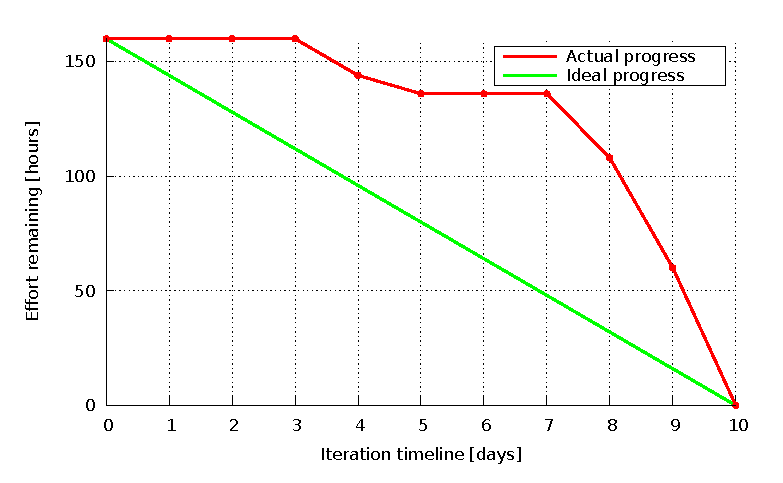
\includegraphics[width=14cm]{burndowns/sprint6.eps}
	\caption{Burn down chart for sprint 6}
	\label{fig:Burn6}
\end{figure}

\subsection{What went well}
It must be noted that the team managed to prepare better for the final demonstration video recording as compared to the last sprint where it only encountered the performance issues for the first time. The devices operated mostly as expected and it was possible to record sufficiently enough video material which was later used for creating the presentation.

\subsection{What could be improved}
The team failed to finish the work within estimated time frame which lead to taking the necessary measures such as working overtime and prioritizing the most important tasks while omitting some less significant ones.
